\documentclass{article}

\usepackage{fancyhdr}
\usepackage{extramarks}
\usepackage{amsmath}
\usepackage{amsthm}
\usepackage{amssymb}
\usepackage{amsfonts}
\usepackage{tikz}
\usepackage{physics}
\usepackage[plain]{algorithm}
\usepackage{algpseudocode}
\usepackage{graphicx,wrapfig,lipsum}
\usetikzlibrary{automata,positioning}

%
% Basic Document Settings
%

\topmargin=-0.45in
\evensidemargin=0in
\oddsidemargin=0in
\textwidth=6.5in
\textheight=9.0in
\headsep=0.25in

\linespread{1.1}

\pagestyle{fancy}
\lhead{\hmwkAuthorName}
\chead{\hmwkClass\ : \hmwkTitle}
\rhead{\firstxmark}
\lfoot{\lastxmark}
\cfoot{\thepage}

\renewcommand\headrulewidth{0.4pt}
\renewcommand\footrulewidth{0.4pt}

\setlength\parindent{0pt}

%
% Create Problem Sections
%
\newcommand{\be}{\begin{equation}}
\newcommand{\ee}{\end{equation}}
\newcommand{\bes}{\begin{equation*}}
\newcommand{\ees}{\end{equation*}}
\newcommand{\bea}{\begin{flalign*}}
\newcommand{\eea}{\end{flalign*}}


\newcommand{\enterProblemHeader}[1]{
    \nobreak\extramarks{}{Problem \arabic{#1} continued on next page\ldots}\nobreak{}
    \nobreak\extramarks{Problem \arabic{#1} (continued)}{Problem \arabic{#1} continued on next page\ldots}\nobreak{}
}

\newcommand{\exitProblemHeader}[1]{
    \nobreak\extramarks{Problem \arabic{#1} (continued)}{Problem \arabic{#1} continued on next page\ldots}\nobreak{}
    \stepcounter{#1}
    \nobreak\extramarks{Problem \arabic{#1}}{}\nobreak{}
}

\setcounter{secnumdepth}{0}
\newcounter{partCounter}
\newcounter{homeworkProblemCounter}
\setcounter{homeworkProblemCounter}{1}
\nobreak\extramarks{Problem \arabic{homeworkProblemCounter}}{}\nobreak{}

%
% Homework Problem Environment
%
% This environment takes an optional argument. When given, it will adjust the
% problem counter. This is useful for when the problems given for your
% assignment aren't sequential. See the last 3 problems of this template for an
% example.
%
\newenvironment{homeworkProblem}[1][-1]{
    \ifnum#1>0
        \setcounter{homeworkProblemCounter}{#1}
    \fi
    \section{Problem \arabic{homeworkProblemCounter}}
    \setcounter{partCounter}{1}
    \enterProblemHeader{homeworkProblemCounter}
}{
    \exitProblemHeader{homeworkProblemCounter}
}

%
% Homework Details
%   - Title
%   - Due date
%   - Class
%   - Section/Time
%   - Instructor
%   - Author
%

\newcommand{\hmwkTitle}{Test\ \#2}
\newcommand{\hmwkDueDate}{Due on 2nd November, 2018}
\newcommand{\hmwkClass}{Fluid Mechanics}
\newcommand{\hmwkClassTime}{}
\newcommand{\hmwkClassInstructor}{}
\newcommand{\hmwkAuthorName}{\textbf{Aditya Vijaykumar}}

%
% Title Page
%

\title{
    %\vspace{2in}
    \textmd{\textbf{\hmwkClass:\ \hmwkTitle}}\\
    \normalsize\vspace{0.1in}\small{\hmwkDueDate\ }\\
%    \vspace{3in}
}

\author{\hmwkAuthorName}
\date{}

\renewcommand{\part}[1]{\textbf{\large Part \Alph{partCounter}}\stepcounter{partCounter}\\}

%
% Various Helper Commands
%

% Useful for algorithms
\newcommand{\alg}[1]{\textsc{\bfseries \footnotesize #1}}

% For derivatives
\newcommand{\deriv}[1]{\frac{\mathrm{d}}{\mathrm{d}x} (#1)}

% For partial derivatives
\newcommand{\pderiv}[2]{\frac{\partial}{\partial #1} (#2)}

% Integral dx
\newcommand{\dx}{\mathrm{d}x}

% Alias for the Solution section header
\newcommand{\solution}{\textbf{\large Solution}}

% Probability commands: Expectation, Variance, Covariance, Bias
\newcommand{\E}{\mathrm{E}}
\newcommand{\Var}{\mathrm{Var}}
\newcommand{\Cov}{\mathrm{Cov}}
\newcommand{\Bias}{\mathrm{Bias}}

\begin{document}

\maketitle


\begin{homeworkProblem}[1]
	\begin{align*}
		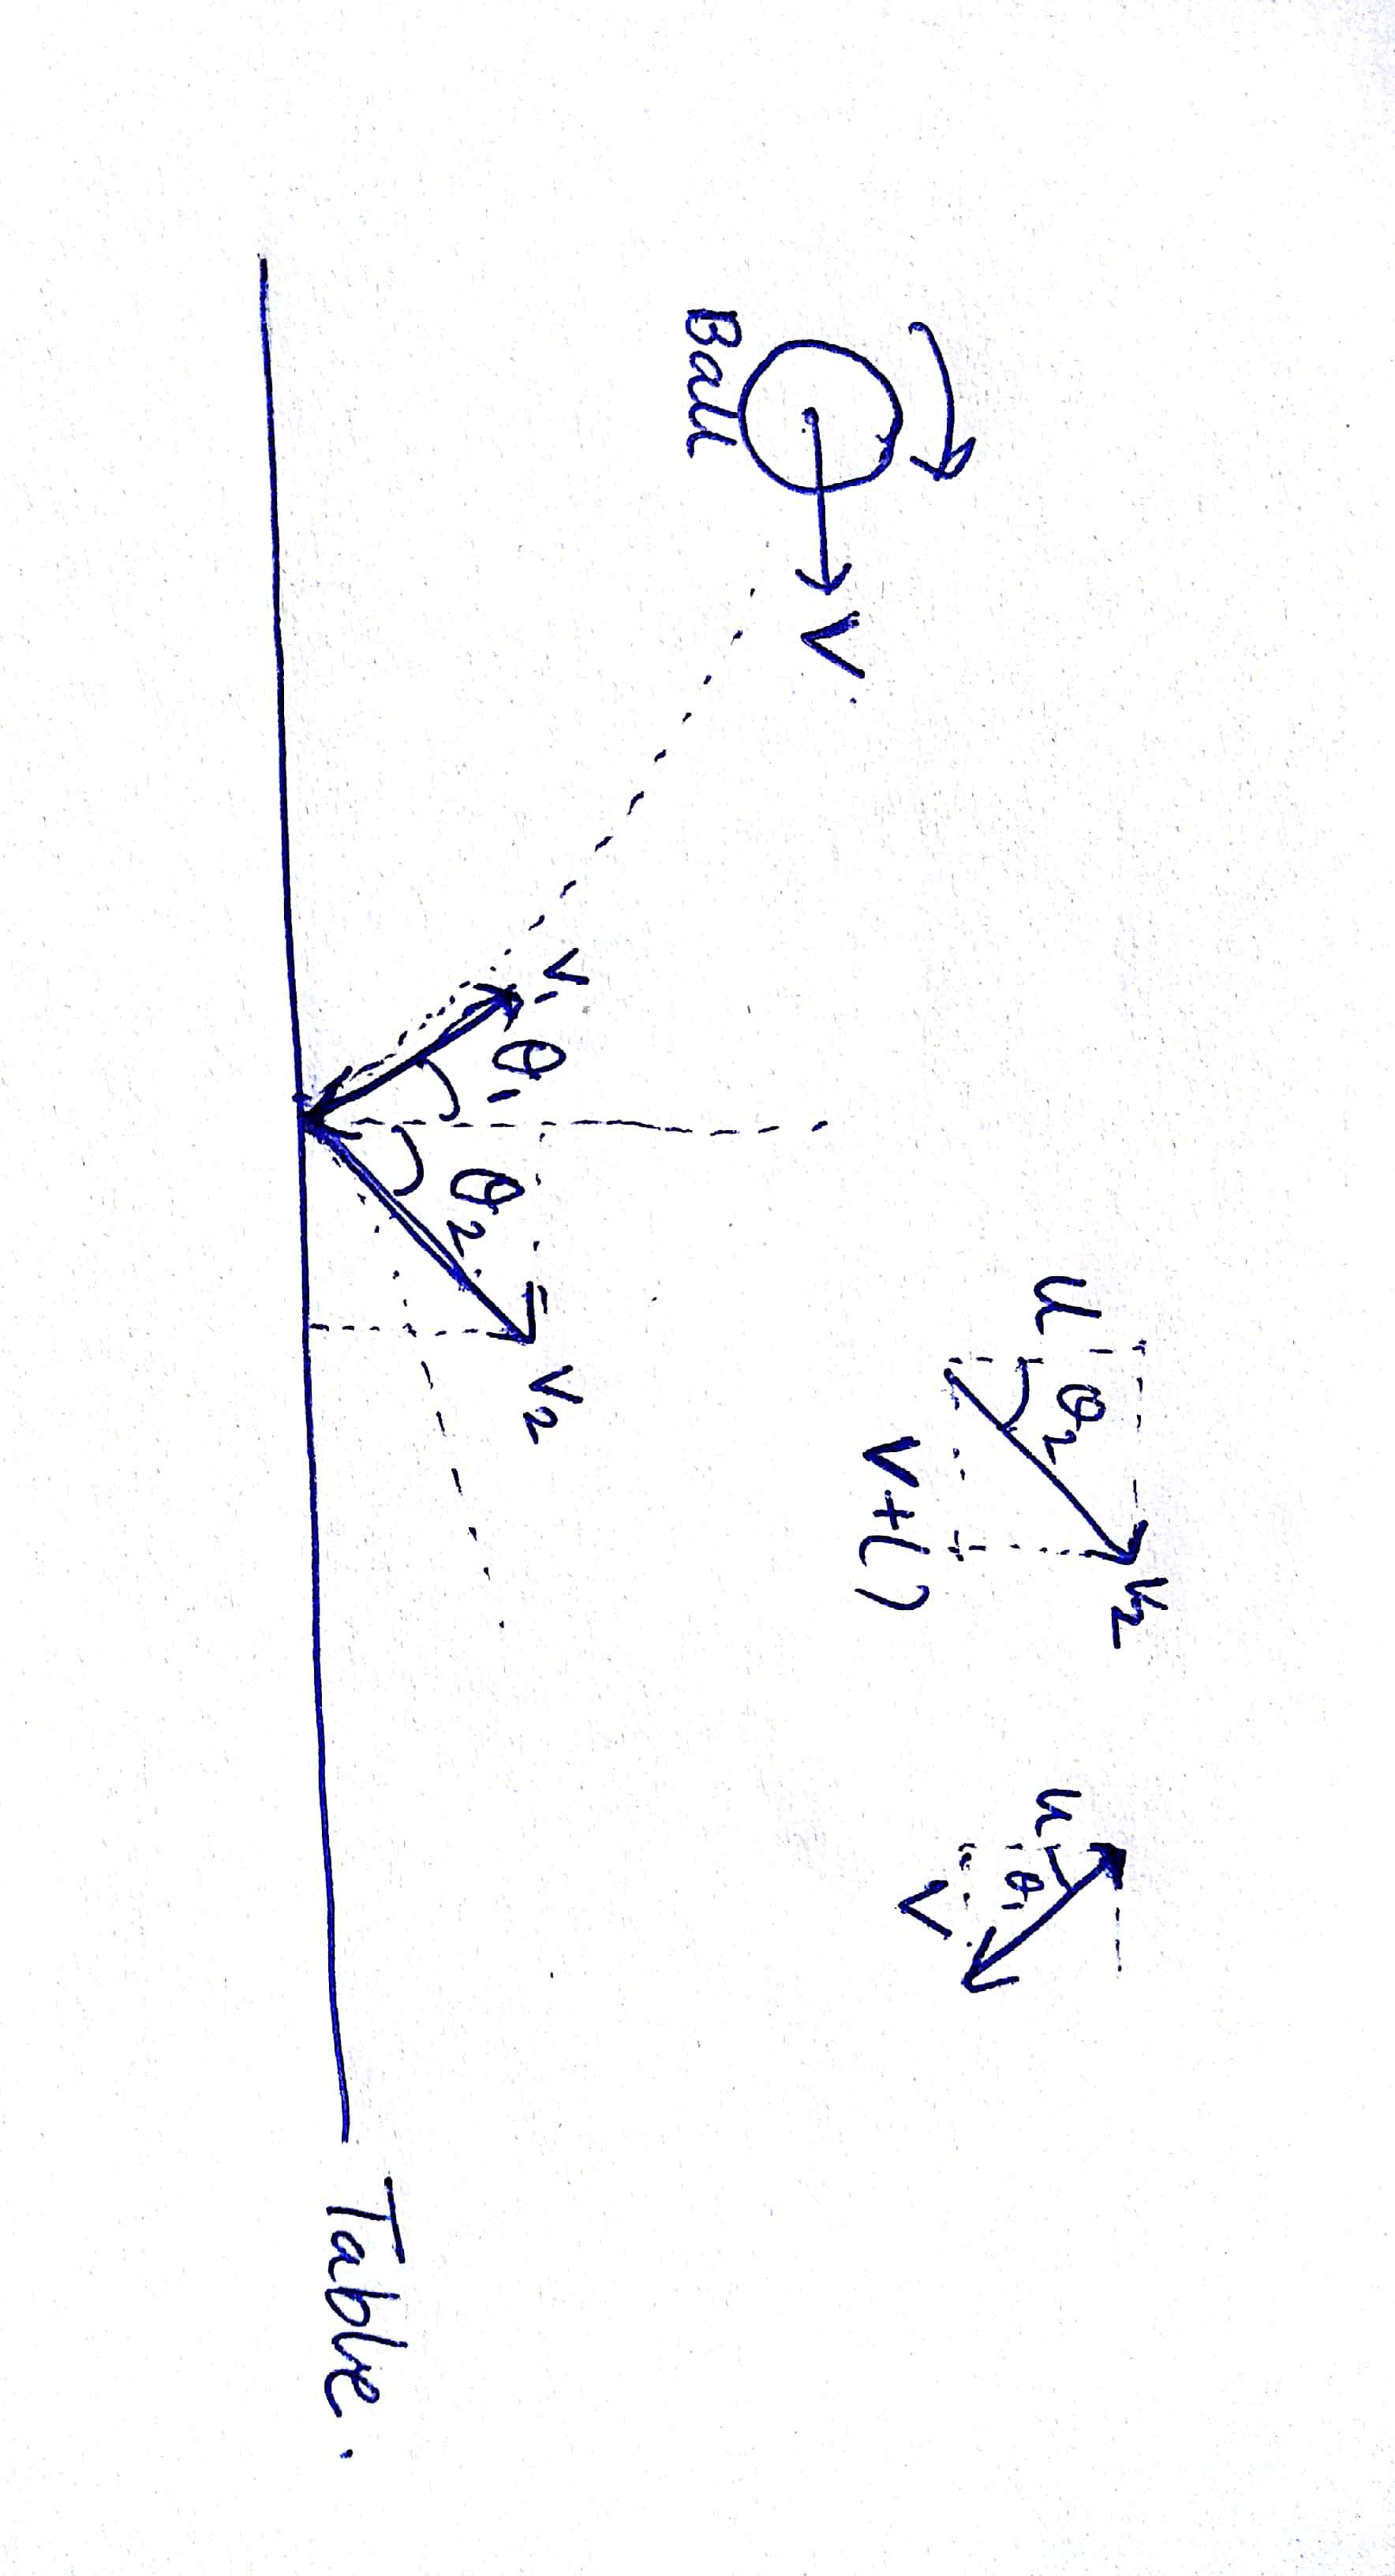
\includegraphics[scale=0.1,angle=90]{q1.jpg}
	\end{align*}
	For the topspin, there will be a corresponding downward force $ \va{L} $ on the ball (assumed to be a cylinder) given by,
	\begin{equation*}
	\va{L} = - \rho V \Gamma \vu{y}
	\end{equation*}
	where $ \rho $ is the density of air and $ \Gamma $ is the circulation strength.
	
	The maximum velocity that can be imparted to the ball is $ V $, and hence the maximum angular velocity imparted is $\frac{V}{R}$, where $ R $ is the radius. So one can find the maximum value of circulation (and consequently maximum lift) from,
	\begin{equation*}
	\dfrac{V}{R} = \dfrac{\Gamma}{2 \pi R^2} \implies \Gamma = {2 \pi R V} \implies \va{L} = -2 \pi \rho R V^2 \vu{y}
	\end{equation*}
	
	We have assumed here that velocity of the player's hand is completely imparted to the ball.
	
	The total force $ \va{F} $ and acceleration $ \va{a} $ acting on the ball is (neglecting air drag),
	\begin{equation*}
	\va{F} = -(mg + 2 \pi \rho R V^2)\vu{y} \implies \va{a} =  -\qty(g + \dfrac{2 \pi \rho R V^2}{m})\vu{y} 
	\end{equation*}
	
	The problem now becomes that of projective motion. If the table is assumed to be at $ y=0 $, and the initial position of the ball is $ (0,H) $, the coordinates $ x $ and $ y $ are given by,
	\begin{equation*}
	x = Vt \qq{,} y = H - \dfrac{1}{2}\qty(g + \dfrac{2 \pi \rho R V^2}{m})t^2
	\end{equation*}
	Note that these formulae for $ x $ and $ y $ are valid only till the time $T$ that the ball first hits the table,
	\begin{equation*}
	 H - \dfrac{1}{2}\qty(g + \dfrac{2 \pi \rho R V^2}{m})T^2 = 0 \implies T = \sqrt{\dfrac{2Hm}{mg + 2 \pi \rho R V^2}}
	\end{equation*}
	The angle that the ball makes with the vertical at the time of collision is,
	\begin{equation*}
	\theta_1 = \tan^{-1}\qty(\dfrac{V}{U}) \qq{;} U=\sqrt{2\qty(g + \dfrac{2 \pi \rho R V^2}{m})H}
	\end{equation*}
	
	On hitting the table, the ball exerts a leftward force on the table, to which there is an equal and rightward reaction force (impulse) acting on the ball. This will increase the net rightward velocity of the ball, and the angle $ \theta_2 $ that the ball makes with the vertical will be greater than $ \theta_1 $
\end{homeworkProblem}



















\begin{homeworkProblem}[2]
	We assume homogenous, isotropic turbulence. These assumptions tell us that the second-order structure function $ S_2 $ calculated between two spatial points should depend \textit{only} on the distance between the two points. More mathematically,
	\begin{equation*}
	\expval{\qty(\va{u}(\va{r} + \va{l}) - \va{u}(\va{r}))^2} = S_2 \qty(\abs{\va{l}}) = S_2(l)
	\end{equation*}
	
	Further, we define the \textit{energy spectrum} $ E(k) $ such that $ E(k)dk $ gives the mean kinetic energy contained within $ k $ and $ k + dk $. It follows from the definition that,
	\begin{equation}
	\int_{0}^{\infty} E(k) dk = \dfrac{1}{2}\expval{u^2}
	\label{ekkin}
	\end{equation}
	The \textit{Wiener-Khinchin} theorem tells us that energy spectrum is the Fourier Transform of the spatial autocorrelation function,
	\begin{equation}
	S_2(l) \sim  \int_{-\infty}^{\infty} e^{i \va{k} \vdot \va{l}} E(k) d^3 \va{k}
	\label{wkt}
	\end{equation}
	
	Now we try to guess the scaling form of $ E(k) $ as $E(k) \sim k^{-n}$. Substituting this ansatz into (\ref{ekkin}),
	\begin{align*}
	\int_{0}^{\infty} E(k) dk &\sim \int_{0}^{\infty} k^{-n} dk \\
	&\sim \eval{\dfrac{k^{1-n}}{1-n}}_{\infty}
	\end{align*}
	As the RHS of (\ref{ekkin}) is finite, it follows from above that $ n > 1 $. We now substitute our ansatz into (\ref{wkt}),
	\begin{align*}
	S_2 (l) &\sim \int_{-\infty}^{\infty} e^{i \va{k} \vdot \va{l}} k^{-n} d^3 \va{k}\\
	&\sim \int_{0}^{\infty}  e^{i kl} k^{-n} dk\int_{0}^{\pi} d(\cos\theta) \int_{0}^{2\pi} d\phi\\
	&\sim \int_{0}^{\infty}  e^{i kl} k^{-n} dk\\
	&\sim \int_{0}^{\infty}  e^{i x} x^{-n} l^n \dfrac{dx}{l} \impliedby \qq{substituting} kl =x \\
	S_2 (l) &\sim \qty[\int_{0}^{\infty} e^{i x} (x)^{-n} dx] l^{n-1}
	\end{align*}
	
	This tells us that $ E(k) \sim k^{-n} \iff S_2(l) \sim l^{n-1}$. In class it was discussed that $ S_2(l) \sim l^{2/3}$ which from the above analysis implies $E(k) \sim k^{-5/3}$. The latter was the expression of the energy spectrum discussed in class.
	
\end{homeworkProblem}



















\begin{homeworkProblem}[3]
	As the depth and the width for all three streams is the same and constant, we expect that at the source on top of the mountain, the volume flow rate $ Q $ gets divided equally between the three streams. Writing unsteady Bernoulli between the topmost point and a point at height $ h $ above the bottom for a given stream $ i $,
	\begin{equation}
	\int \rho \pdv{v_i}{t} ds + \qty(P_{atm} + \dfrac{\rho Q^2}{18 A^2} + \rho g H) - \qty(P_{atm} + \dfrac{\rho v_i^2}{2} + \rho g h)
	\label{uparneeche}
	\end{equation}
	where the integral is along a streamline. The path of the water can be given as,
	\begin{equation*}
	ds = \sqrt{dx_i^2 + dy_i^2} = dh\sqrt{\dot{x}_i^2 + \dot{y}_i^2} \qq{where} \dot{x}_i= \dv{x_i}{h} \qq{and} \dot{y}_i = \dv{y_i}{h}
	\end{equation*}
	We denote the distance that the water has travelled by $ L_i(h) $,
	\begin{equation*}
	L_i(h) = \abs{\int_H^{h} dh \sqrt{\dot{x}_i^2 + \dot{y}_i^2}}
	\end{equation*}
	So we can then rewrite (\ref{uparneeche}) as,
	\begin{equation*}
	\pdv{v_i}{t} L_i(h) = -\qty(\dfrac{v_i^2}{2} - \dfrac{Q^2}{18A^2} - \rho g (H-h)) \implies \pdv{v_i}{t} = -\dfrac{9A^2 v_i^2 - Q^2 - 18g(H-h)A^2}{18A^2L_i(h)}
	\end{equation*}
	Using $\alpha(h)^2 = \dfrac{Q^2 + 18g(H-h)A^2}{9A^2}$
	\begin{equation*}
	\dfrac{1}{2\alpha(h)} \ln \dfrac{v_i- \alpha}{v_i + \alpha} = - \dfrac{\alpha(h) t}{L_i(h)} \implies v_i(t,h) = \alpha(h) \tanh\dfrac{\alpha(h) t}{2L_i(h)}
	\end{equation*}
\end{homeworkProblem}













\end{document}
